\documentclass[12pt]{article}

% ========== PACKAGES ==========
\usepackage{amsmath}          % For advanced math environments
\usepackage{amssymb}          % For math symbols
\usepackage{graphicx}         % To include images
\usepackage[a4paper, margin=1in]{geometry} % For page layout
\usepackage{xcolor}           % For colors
\usepackage{hyperref}         % For hyperlinks
\usepackage{fancyhdr}         % For headers and footers
\usepackage{tikz}             % For drawing diagrams
\usepackage{siunitx}          % For typesetting units correctly
\usepackage{gensymb}          % Provides the \degree symbol, used with siunitx

% ========== TIKZ LIBRARIES ==========
\usetikzlibrary{decorations.pathmorphing}
\usetikzlibrary{arrows.meta}

% ========== DOCUMENT INFORMATION ==========
\title{Teaching Notes \& Solved Problems: Thermal Conductivity}
\author{Gemini AI}
\date{\today}

% ========== HEADER AND FOOTER ==========
\pagestyle{fancy}
\fancyhf{}
\rhead{Thermal Conductivity}
\lhead{\thetitle}
\cfoot{\thepage}

\begin{document}

\maketitle
\thispagestyle{empty}
\tableofcontents
\newpage

\section{Teaching Notes: Thermal Conductivity (1-Hour Lesson)}

\subsection{Part 1: The Basics of Heat Conduction (15 mins)}

\subsubsection*{What is Heat Conduction?}
Heat conduction is the transfer of thermal energy through a substance by the collision of its constituent particles (atoms, molecules, electrons).
\begin{itemize}
    \item In \textbf{solids}, atoms vibrate in fixed positions and pass energy to their neighbors. In metals, free-moving electrons also carry energy, making them excellent conductors.
    \item Conduction is one of the three modes of heat transfer, along with \textbf{convection} (heat transfer by fluid movement) and \textbf{radiation} (heat transfer by electromagnetic waves).
\end{itemize}

\subsubsection*{Fourier's Law of Heat Conduction}
The fundamental equation for heat conduction is Fourier's Law. For a uniform object like a rod, the rate of heat flow ($P$) is given by:
$$P = \frac{dQ}{dt} = \frac{kA(T_H - T_C)}{L}$$
Let's break down the terms:
\begin{itemize}
    \item \textbf{$P$}: The \textbf{rate of heat flow} (heat current), in \si{\watt} (\si{\joule\per\second}).
    \item \textbf{$k$}: The \textbf{thermal conductivity} of the material, in \si{\watt\per\meter\per\kelvin}. High $k$ means a good conductor; low $k$ means a good insulator.
    \item \textbf{$A$}: The \textbf{cross-sectional area} through which heat flows, in \si{\meter\squared}. For a cylinder, $A = \pi r^2$.
    \item \textbf{$T_H$} and \textbf{$T_C$}: The temperatures of the \textbf{hot} and \textbf{cold} ends.
    \item \textbf{$L$}: The \textbf{length} of the material, in \si{\meter}.
\end{itemize}

% Diagram of Heat Conduction
\begin{figure}[h!]
\centering
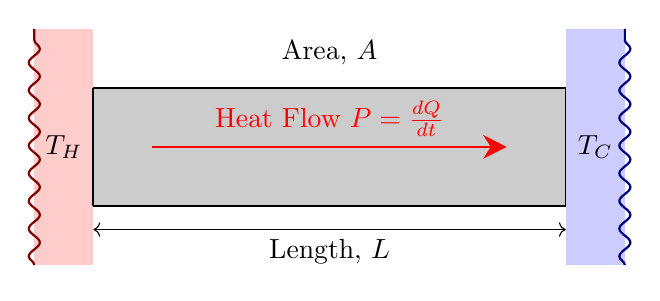
\begin{tikzpicture}[scale=1.5]
    % Hot Reservoir
    \fill[red!20] (-0.5, -1) rectangle (0, 1);
    \draw[red!50!black, thick, decoration={snake, segment length=10pt, amplitude=2pt}, decorate] (-0.5, -1) -- (-0.5, 1);
    \node at (-0.25, 0) {$T_H$};
    
    % Rod
    \fill[gray!40] (0, -0.5) rectangle (4, 0.5);
    \draw[thick] (0, -0.5) -- (4, -0.5);
    \draw[thick] (0, 0.5) -- (4, 0.5);
    \draw[thick] (0, -0.5) -- (0, 0.5);
    \draw[thick] (4, -0.5) -- (4, 0.5);

    % Heat Flow Arrow
    \draw[-{Stealth[length=3mm, width=3mm]}, red, thick] (0.5, 0) -- (3.5, 0) node[midway, above] {Heat Flow $P = \frac{dQ}{dt}$};
    
    % Cold Reservoir
    \fill[blue!20] (4, -1) rectangle (4.5, 1);
    \draw[blue!50!black, thick, decoration={snake, segment length=10pt, amplitude=2pt}, decorate] (4.5, -1) -- (4.5, 1);
    \node at (4.25, 0) {$T_C$};
    
    % Labels
    \draw[<->] (0, -0.7) -- (4, -0.7) node[midway, below] {Length, $L$};
    \node at (2, 0.8) {Area, $A$};
\end{tikzpicture}
\caption{Heat conduction through a uniform rod from a hot reservoir to a cold reservoir.}
\label{fig:conduction}
\end{figure}

\subsection{Part 2: Applying the Concept (15 mins)}

\subsubsection*{Connecting to Other Thermal Concepts}
The heat ($Q$) transferred by conduction can cause:
\begin{enumerate}
    \item \textbf{Phase Changes (Latent Heat):} To change a substance's state (e.g., melt ice) at a constant temperature.
    \[ Q = m L_f \]
    The rate of mass melting is related to the rate of heat flow: $P = \frac{dQ}{dt} = L_f \frac{dm}{dt}$.

    \item \textbf{Temperature Changes (Specific Heat Capacity):} To change a substance's temperature.
    $$Q = mc\Delta T$$
\end{enumerate}

\newpage
\section{Solutions to Provided Problems}

\subsection{Problem 1 (SPhO 2022)}
\subsubsection*{Question Text}
\begin{quote}
A well-lagged uniform cylindrical rod is \SI{20.0}{\centi\meter} long and has a diameter of \SI{2.00}{\centi\meter}. One end of it is in thermal contact with a hot reservoir maintained at a temperature of \SI{150}{\celsius} while the other end is in thermal contact with a very large block of ice at temperature \SI{0}{\celsius}.
(i) It is found that the ice block is melting at a rate of \SI{0.1683}{\kilogram\per\minute}. What is the thermal conductivity of the material of the rod?
(ii) Calculate the rate of change of the entropy of the system comprising the hot and cold reservoirs and the rod.
[Latent heat of fusion of ice $= \SI{3.36e4}{\joule\per\kilogram}$]
\end{quote}

\subsubsection*{Solution (i): Thermal Conductivity}
\begin{enumerate}
    \item \textbf{Calculate the rate of heat flow ($P$)}: The heat transferred melts the ice. Convert the rate of melting to \si{\kilogram\per\second}.
    \[ \frac{dm}{dt} = \SI{0.1683}{\kilogram\per\minute} \times \frac{\SI{1}{\minute}}{\SI{60}{\second}} = \SI{0.002805}{\kilogram\per\second} \]
    Use the latent heat of fusion to find the power.
    \[ P = L_f \frac{dm}{dt} = (\SI{3.36e4}{\joule\per\kilogram}) \times (\SI{0.002805}{\kilogram\per\second}) = \SI{94.248}{\watt} \]
    
    \item \textbf{Gather parameters}:
    \begin{itemize}
        \item Length, $L = \SI{20.0}{\centi\meter} = \SI{0.200}{\meter}$
        \item Diameter = \SI{2.00}{\centi\meter}, so radius, $r = \SI{1.00}{\centi\meter} = \SI{0.0100}{\meter}$
        \item Area, $A = \pi r^2 = \pi (\SI{0.0100}{\meter})^2 = \pi \times 10^{-4} \, \si{\meter\squared}$
        \item Temp. difference, $\Delta T = \SI{150}{\celsius} - \SI{0}{\celsius} = \SI{150}{\kelvin}$
    \end{itemize}

    \item \textbf{Solve for thermal conductivity ($k$)}:
    \begin{align*}
        P &= \frac{kA\Delta T}{L} \\
        k &= \frac{PL}{A\Delta T} = \frac{(\SI{94.248}{\watt})(\SI{0.200}{\meter})}{(\pi \times 10^{-4} \, \si{\meter\squared})(\SI{150}{\kelvin})} \\
        k &\approx \SI{400}{\watt\per\meter\per\kelvin}
    \end{align*}
\end{enumerate}

\subsubsection*{Solution (ii): Rate of Entropy Change}
The total rate of entropy change is $\frac{dS_{\text{total}}}{dt} = \frac{dS_{\text{hot}}}{dt} + \frac{dS_{\text{cold}}}{dt} + \frac{dS_{\text{rod}}}{dt}$. For a reservoir, $\frac{dS}{dt} = \frac{P}{T}$. Since the rod is in steady state, $\frac{dS_{\text{rod}}}{dt} = 0$. Temperatures must be in Kelvin:
\begin{itemize}
    \item $T_H = \SI{150}{\celsius} + 273.15 = \SI{423.15}{\kelvin}$
    \item $T_C = \SI{0}{\celsius} + 273.15 = \SI{273.15}{\kelvin}$
\end{itemize}
\begin{enumerate}
    \item \textbf{Hot reservoir (loses heat)}:
    \[ \frac{dS_{\text{hot}}}{dt} = \frac{-P}{T_H} = \frac{-\SI{94.248}{\watt}}{\SI{423.15}{\kelvin}} = \SI{-0.2227}{\joule\per\kelvin\per\second} \]
    \item \textbf{Cold reservoir (gains heat)}:
    \[ \frac{dS_{\text{cold}}}{dt} = \frac{+P}{T_C} = \frac{+\SI{94.248}{\watt}}{\SI{273.15}{\kelvin}} = \SI{+0.3451}{\joule\per\kelvin\per\second} \]
    \item \textbf{Total entropy change}:
    \[ \frac{dS_{\text{total}}}{dt} = -0.2227 + 0.3451 = \SI{0.1224}{\joule\per\kelvin\per\second} \]
\end{enumerate}

\newpage
\subsection{Problem 2 (SPhO 2020)}
\subsubsection*{Question Text}
\begin{quote}
One end of a copper rod, with diameter \SI{2.0}{\centi\meter} and length \SI{50.0}{\centi\meter}, is in good thermal contact with a hot bath maintained at \SI{100}{\celsius} while the other end is immersed in a mixture of \SI{200}{\gram} ice and \SI{100}{\gram} water initially maintained at \SI{0}{\celsius} inside a container whose thermal capacity is negligible. Both the copper rod and the container are well-lagged. How long does it take for the temperature of the mixture to rise from \SI{0}{\celsius} to \SI{20}{\celsius}?
[Thermal conductivity of copper $= \SI{400}{\watt\per\meter\per\kelvin}$
Specific heat capacity of water $= \SI{4200}{\joule\per\kilogram\per\kelvin}$
Latent heat of fusion of water $= \SI{3.34e5}{\joule\per\kilogram}$]
\end{quote}

\subsubsection*{Solution}
This is a two-stage process. First, melt the ice, then heat the water.
\paragraph{Parameters:}
\begin{itemize}
    \item $k = \SI{400}{\watt\per\meter\per\kelvin}$
    \item $L = \SI{50.0}{\centi\meter} = \SI{0.50}{\meter}$
    \item $A = \pi r^2 = \pi(\SI{0.01}{\meter})^2 = \pi \times 10^{-4} \, \si{\meter\squared}$
    \item $T_H = \SI{100}{\celsius}$
    \item $m_{\text{ice}} = \SI{0.2}{\kilogram}$, $m_{\text{water, initial}} = \SI{0.1}{\kilogram}$
\end{itemize}

\subsubsection*{Stage 1: Melting the ice (Time $t_1$)}
The cold end remains at $T_C = \SI{0}{\celsius}$. The rate of heat flow is constant.
\begin{enumerate}
    \item \textbf{Heat required ($Q_1$)}:
    \[ Q_1 = m_{\text{ice}} L_f = (\SI{0.2}{\kilogram})(\SI{3.34e5}{\joule\per\kilogram}) = \SI{66800}{\joule} \]
    \item \textbf{Rate of heat flow ($P_1$)}:
    \[ P_1 = \frac{kA(T_H - T_C)}{L} = \frac{(400)(\pi \times 10^{-4})(100 - 0)}{0.50} = 80\pi \, \si{\watt} \approx \SI{251.3}{\watt} \]
    \item \textbf{Time taken ($t_1$)}:
    \[ t_1 = \frac{Q_1}{P_1} = \frac{66800}{80\pi} \approx \SI{265.8}{\second} \]
\end{enumerate}

\subsubsection*{Stage 2: Heating the water from \SI{0}{\celsius} to \SI{20}{\celsius} (Time $t_2$)}
The temperature of the cold end, $T_C(t)$, now increases. The total mass of water is $m_{\text{total}} = \SI{0.3}{\kilogram}$.
\begin{enumerate}
    \item \textbf{Set up the differential equation}:
    The heat $dQ$ flowing into the water raises its temperature by $dT_C$.
    \[ dQ = m_{\text{total}} c_w dT_C \]
    This heat is supplied by the rod at a non-constant rate:
    \[ \frac{dQ}{dt} = \frac{kA(T_H - T_C(t))}{L} \]
    Equating the two expressions for $dQ$:
    \[ m_{\text{total}} c_w dT_C = \frac{kA(T_H - T_C)}{L} dt \]
    
    \item \textbf{Separate variables and integrate}:
    \[ dt = \frac{m_{\text{total}} c_w L}{kA} \frac{dT_C}{T_H - T_C} \]
    \[ \int_0^{t_2} dt = \frac{m_{\text{total}} c_w L}{kA} \int_{0}^{20} \frac{dT_C}{100 - T_C} \]
    The integral is $[-\ln(100 - T_C)]$.
    \begin{align*}
        t_2 &= \frac{m_{\text{total}} c_w L}{kA} \left[-\ln(100 - T_C)\right]_{0}^{20} \\
        t_2 &= \frac{m_{\text{total}} c_w L}{kA} \left(-\ln(80) - (-\ln(100))\right) \\
        t_2 &= \frac{m_{\text{total}} c_w L}{kA} \ln\left(\frac{100}{80}\right) = \frac{(\SI{0.3}{})(\SI{4200}{})(\SI{0.5}{})}{(400)(\pi \times 10^{-4})} \ln(1.25) \\
        t_2 &= \frac{630}{0.04\pi} \ln(1.25) \approx (5013.2)(0.2231) \approx \SI{1118.6}{\second}
    \end{align*}
\end{enumerate}

\subsubsection*{Total Time}
The total time is the sum of the times for both stages.
\[ t_{\text{total}} = t_1 + t_2 = \SI{265.8}{\second} + \SI{1118.6}{\second} = \SI{1384.4}{\second} \]
This is approximately $\mathbf{23.1}$ minutes.

\end{document}